\entry{2026-10-18}{3D speed lane (complete): speed-up over our own baselines, but the spectral FOM wins (K2 fires)}

Lane \texttt{2026-10-14-jcp-speed3d}, last commit \texttt{691465d88}, mirror \texttt{6c270e6c5}. The lane was resumed by the Burgers campaign coordinator after its first agent stopped. Jobs on H200 (all \texttt{jax\_backend=gpu}): g1 5301580, g2 5301264, g3 5301270, f1 5301274, p1 5352455, m1 5352457, r1 5353792; 10.9 of 34 GPU-h. Namespace emptied. Final report audit READY. Numbers are quoted from the generated \path{report.md}; errors are against E0 $R_{ST}$ (a conditional Richardson estimate).

\begin{itemize}
\item \textbf{Speed over our earlier 3D configurations (H2, bar $1.67\times$, paired panels):} pass against all three. 2.01$\times$ vs the old deployment, 5.37$\times$ vs W768, 17.2$\times$ vs W1024. The winners use the narrower M2\_512 bank with Gauss $24^3$ and second-order stepping (BDF2 one-pass or quasi-Newton CN).
\item \textbf{Cost is flat in the mesh (H4.1):} the online solve time changes by at most a factor 1.007--1.09 from $64^3$ to $384^3$ for all four ROMs (mesh-free query; deployment mode policy). Coordinator recheck from raw m1 timings: 1.004--1.098, same verdict.
\item \textbf{Against the full simulation: K2 fires.} At $384^3$, no selected ROM reaches $2\times$ against the best matched FOM across families; against that union the ROMs run at 0.008--0.16$\times$ the FOM's speed. A pseudo-spectral FOM at $N=16$ matches the ROM's accuracy. Against central-CN only, one ROM reaches 2.03$\times$. Matched speed-ups are upper bounds (finite FOM ladder).
\item \textbf{The early observation} ``spectral FOM clearly beats the ROM at $64^3$'' is \textbf{confirmed}.
\item Replication on cohort 923901: all three winners hold (2.03$\times$, 5.31$\times$, 16.6$\times$).
\end{itemize}
\begin{center}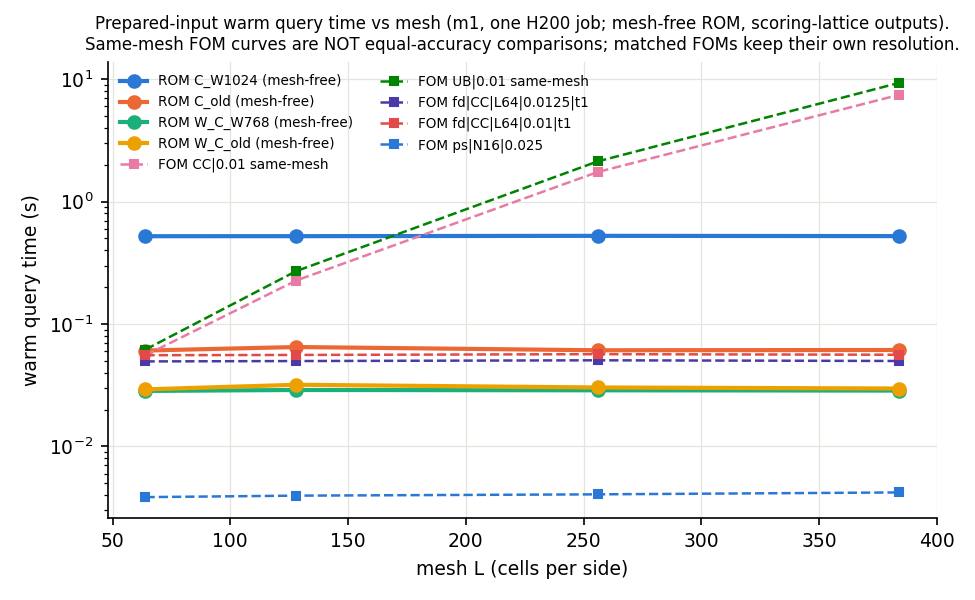
\includegraphics[width=0.48\linewidth]{figs/s3_mesh_time.png}\hfill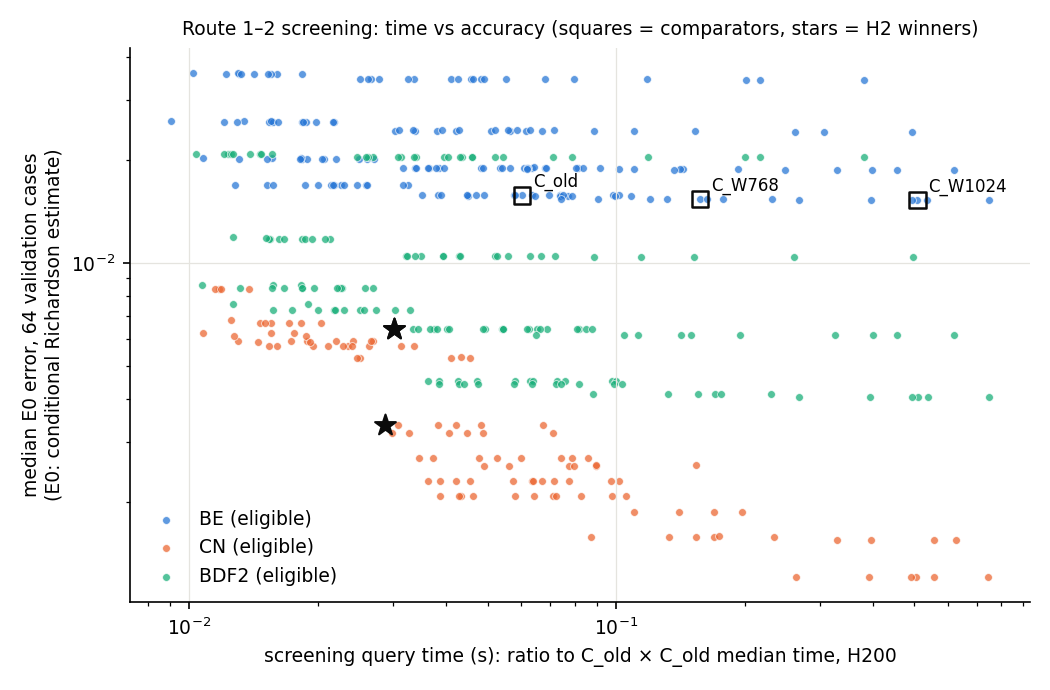
\includegraphics[width=0.48\linewidth]{figs/s3_pareto.png}\end{center}

\subsection*{Consequence for the paper}
Following the plan's written consequence for K2: report the speed-up honestly (no win over the spectral FOM in 3D Burgers on the box) and lead with mesh-independence of cost. The upwind FOM cells are undecided (no upwind ladder member is as accurate as the ROM).

\subsection*{Corrections}
\retracted{A9's attribution of the G2 failures was wrong (corrected in A10). G2 fails literally on 15 of 288{,}944 steps, all at $\gamma\le3.4\times10^{-12}$; no classification changes. The m1 calibration population and the L256 resource estimate were corrected before results were read. The flat-cost result holds for the deployment mode policy, not for a fixed test space (no fixed-mode panel ran). Replication eligibility is not a fresh Q1 certificate.}
